
\renewcommand{\EntradaBibtex}{PaseListasCodigoQRFaceDetection_SistemasInteligentes_UPV_2024}

\begin{frame}{\citetitle{\EntradaBibtex}$^*$ (1)}
\begin{block}{Motivación} 
Se requiere una herramienta que permita efectuar un pase de lista efectivo en grupos numerosos. 
\begin{itemize}
\item Se capturan fotografias de los asistentes del grupo, además de asignar a cada alumno de un código QR
\item Se emplea un modelo un módulo de Python denominado \textit{face-recognition} para entrena un modelo de aprendizaje profundo para reconocer los rostros de los asistentes a la clase
\item Se emplea una librería para detección de códigos QR
\item Se cruza la información de la identidad del estudiante con el código QR
\end{itemize}
\end{block} 
\footfullcite*{\EntradaBibtex}
\end{frame}


\begin{frame}{\citetitle{\EntradaBibtex} (2)}
%\begin{block}{Pantallas Principales} 

%\begin{columns}
% Column 1
%\column{.1\linewidth}
%\begin{center}
%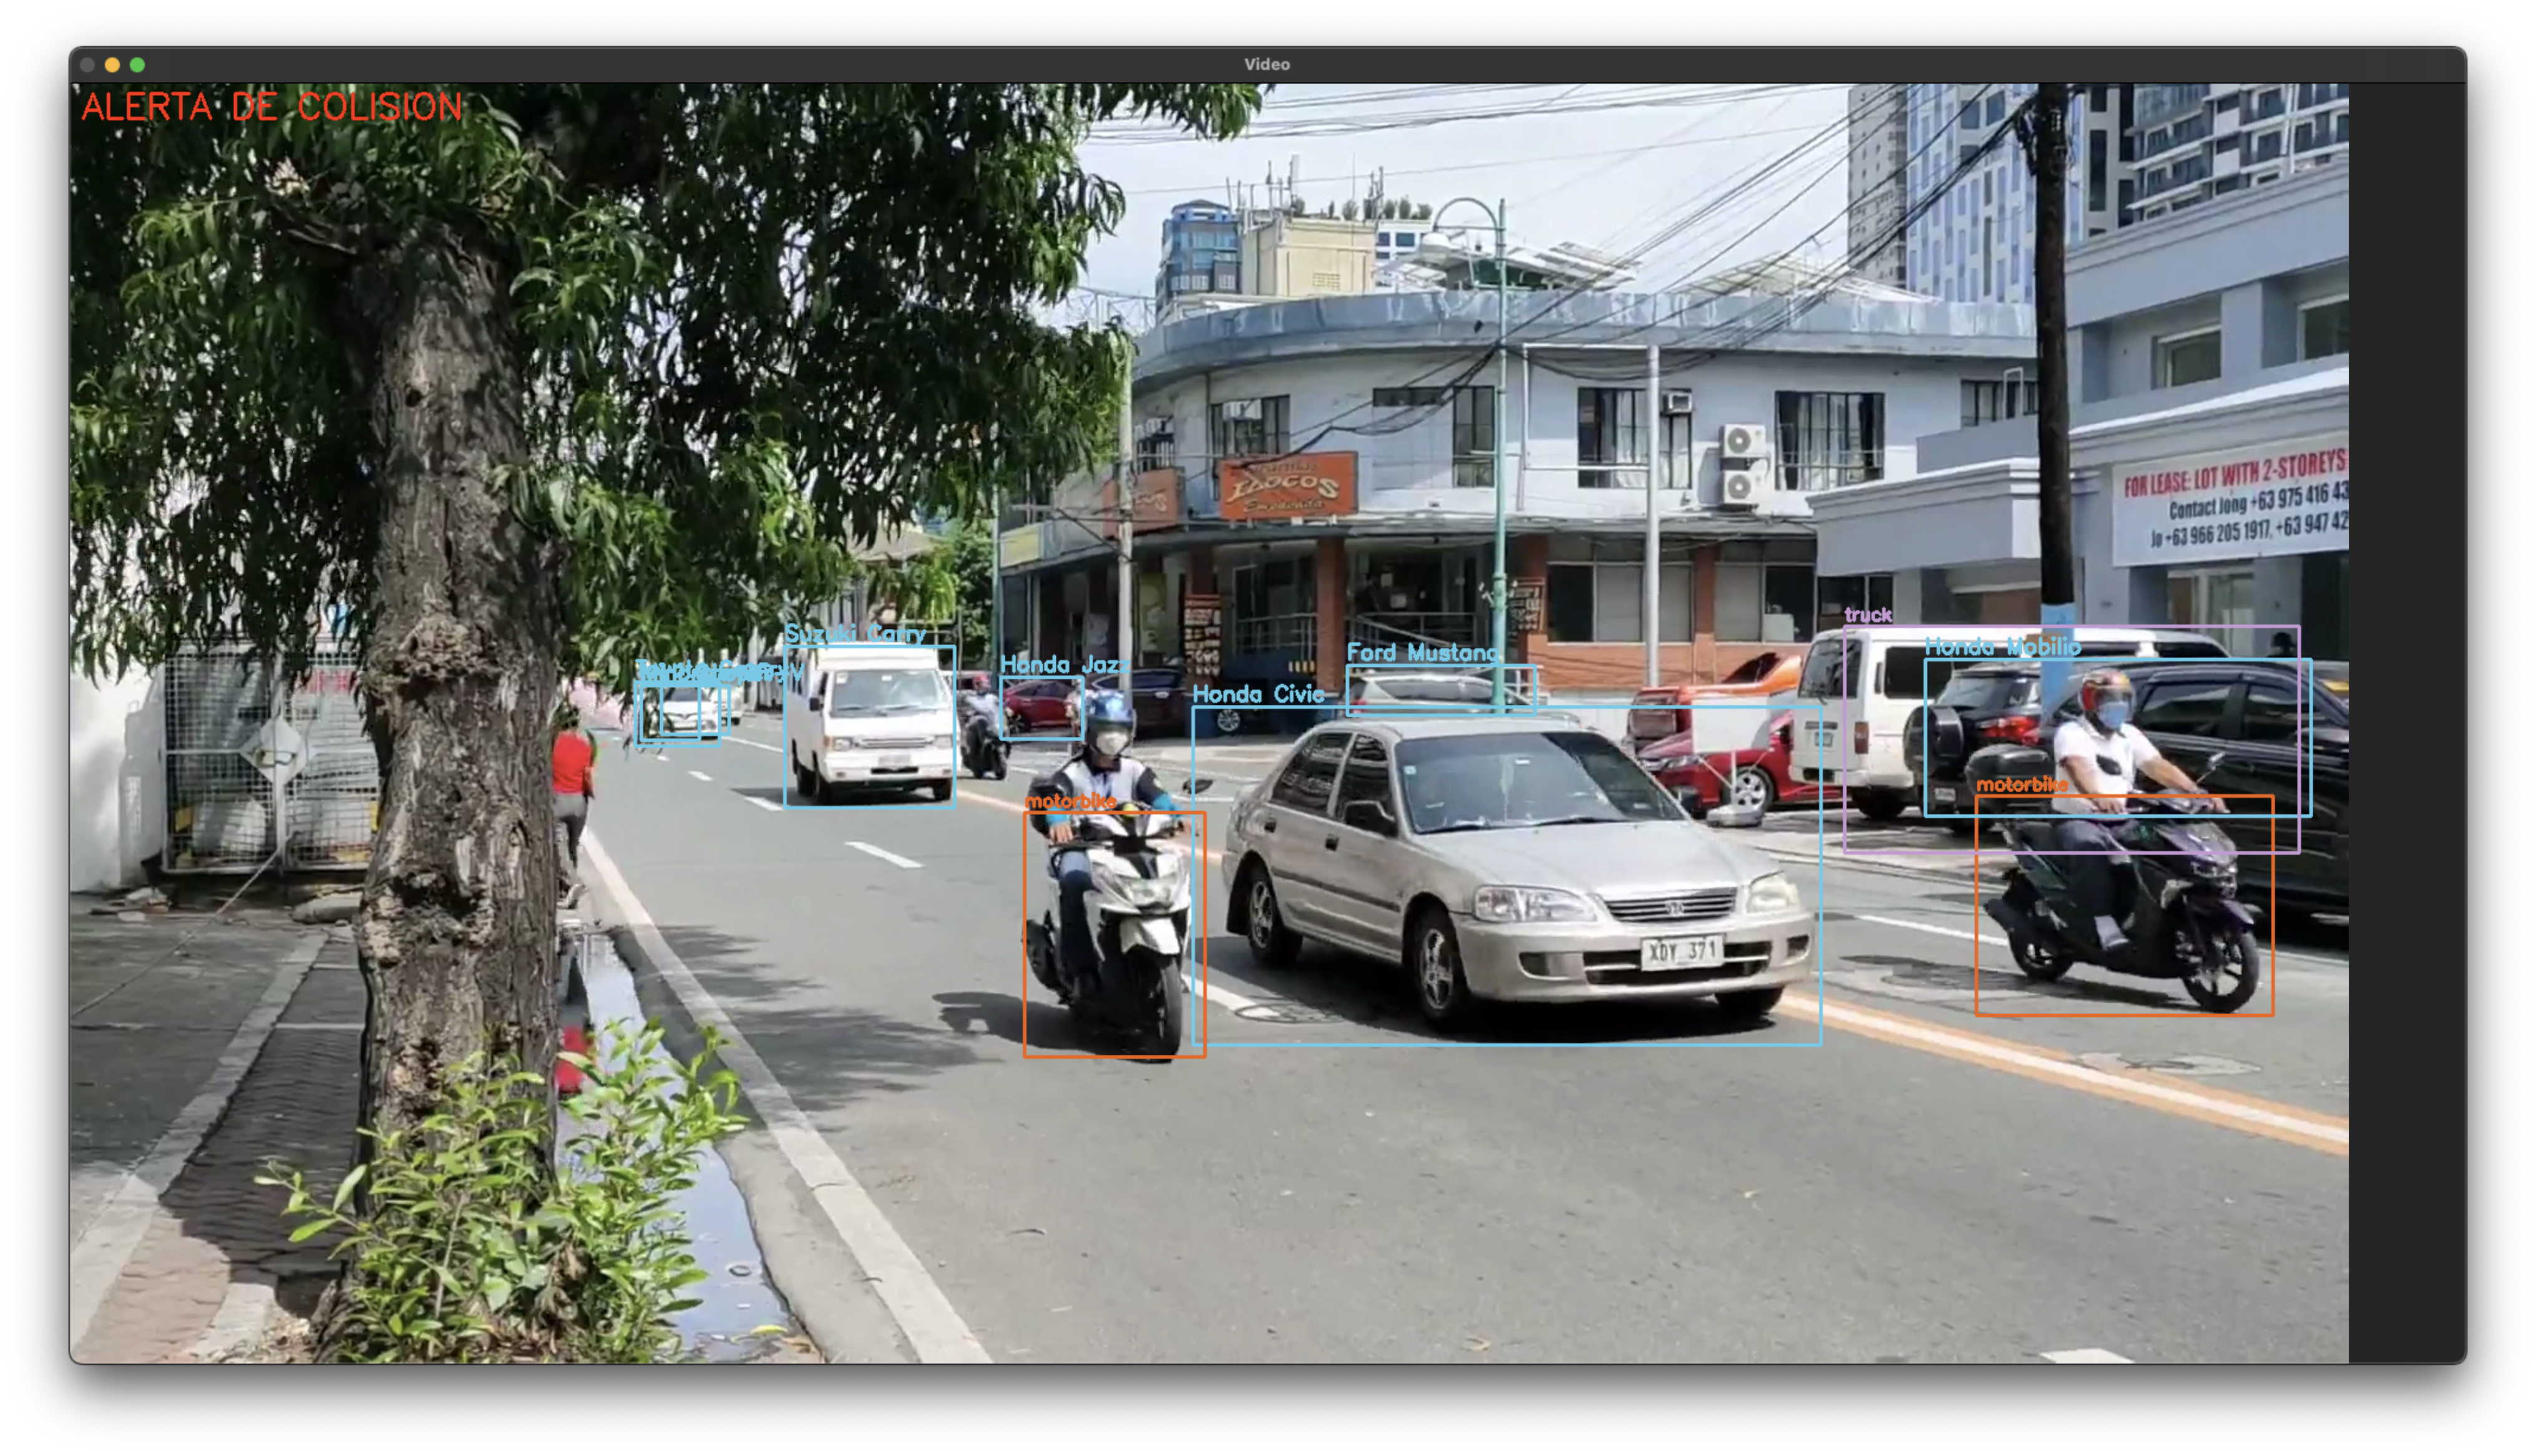
\includegraphics[width=0.85\linewidth]{2024_DetectorMotos/figs/resultados1.png}
%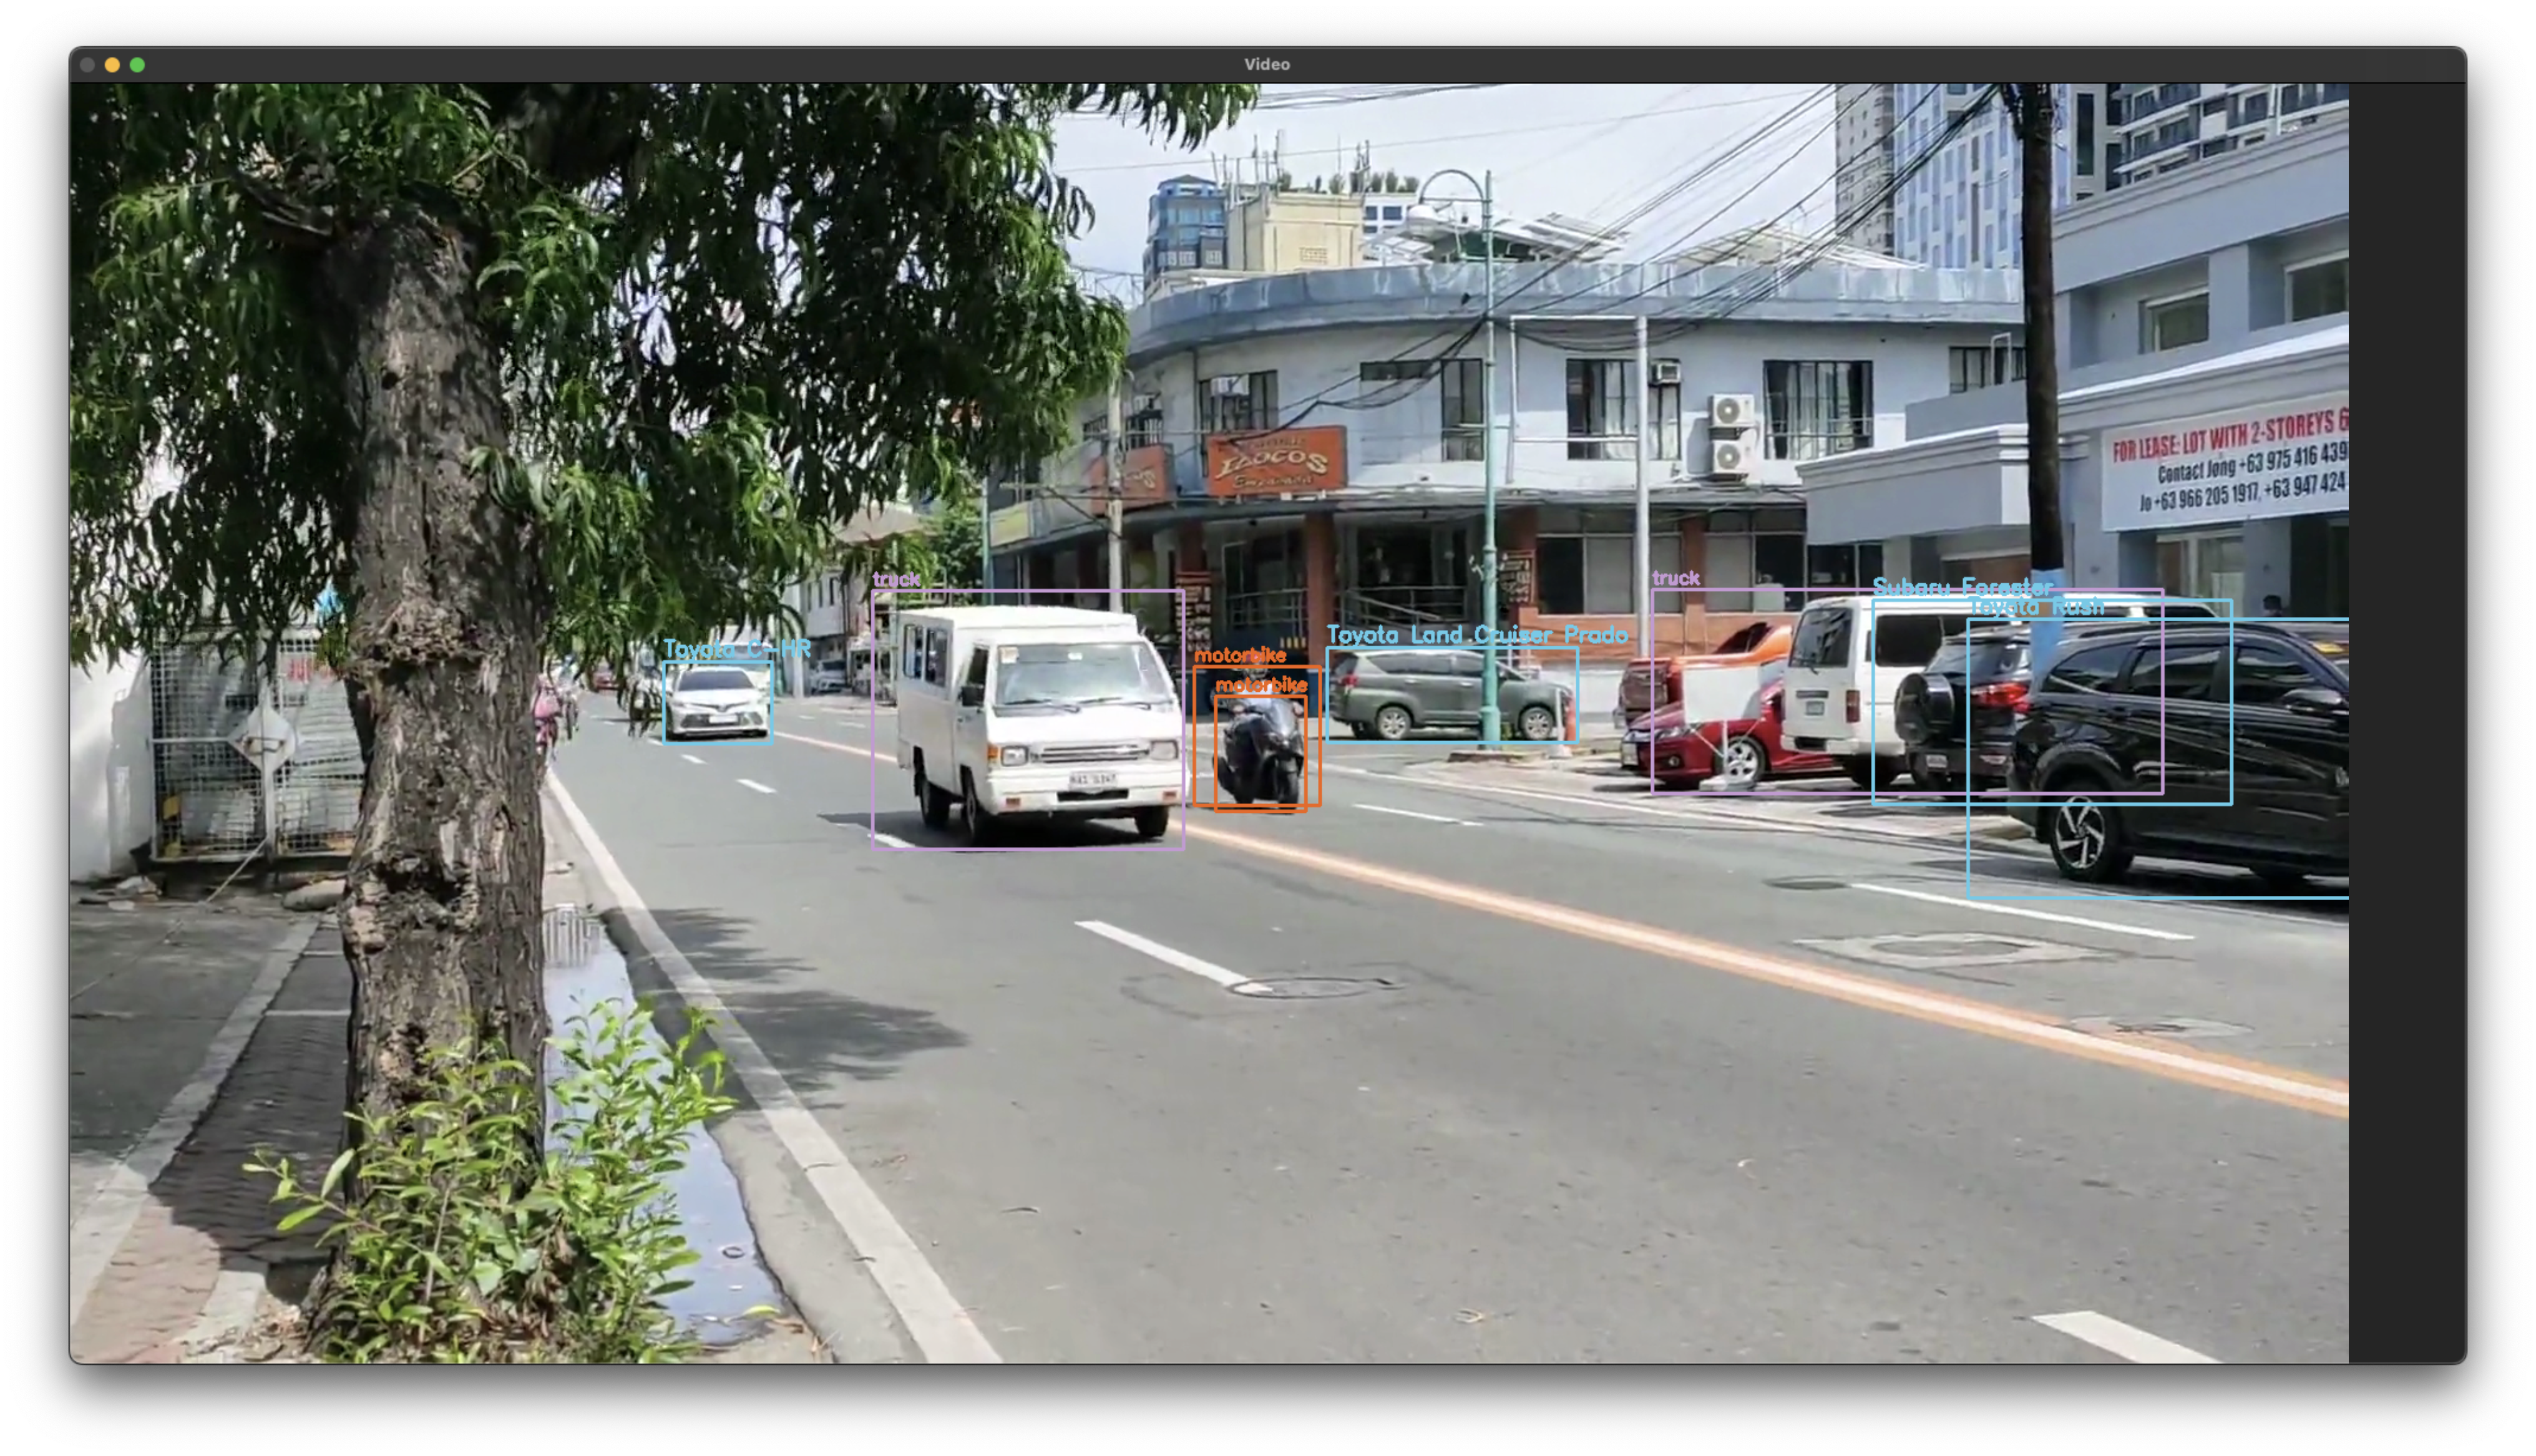
\includegraphics[width=0.85\linewidth]{2024_DetectorMotos/figs/resultados2.png}
%\end{center}
%\column{.9\linewidth}
\begin{center}
	\begin{tabular}{ccc}
		\includegraphics[width=0.20\linewidth]{2024_PaseDeListaCodigoQR/figs/2.jpg} &
		\includegraphics[width=0.38\linewidth]{2024_PaseDeListaCodigoQR/figs/3.jpg} &
 		\includegraphics[width=0.38\linewidth]{2024_PaseDeListaCodigoQR/figs/4.jpg} \\
	\end{tabular}
\end{center}

%\end{columns}
\end{frame}

%/media/marco/Master/00_0A0RespadoLaptopHP_2024/Escritorio/00_DiapositivasProyectos/2024_PaseDeListaCodigoQR/figs/2.jpg
%/media/marco/Master/00_0A0RespadoLaptopHP_2024/Escritorio/00_DiapositivasProyectos/2024_PaseDeListaCodigoQR/figs/3.jpg
%/media/marco/Master/00_0A0RespadoLaptopHP_2024/Escritorio/00_DiapositivasProyectos/2024_PaseDeListaCodigoQR/figs/4.jpg


